\documentclass[11pt,a4paper]{article}

% ==============================================================================
% PACKAGES & TYPOGRAPHY (XeLaTeX)
% ==============================================================================
\usepackage{fontspec}
\setmainfont{Times New Roman}
\setsansfont{Arial}

\usepackage[top=2.2cm, bottom=2.2cm, left=2.3cm, right=2.3cm, headheight=28pt]{geometry}
\setlength{\emergencystretch}{2.5em}
\tolerance=800
\usepackage{graphicx}
\usepackage{xcolor}
\usepackage{colortbl}
\usepackage{booktabs}
\usepackage{tabularx}
\usepackage{longtable}
\usepackage{array}
\usepackage{multirow}
\usepackage{float}
\usepackage{enumitem}
\usepackage{titlesec}
\usepackage[titles]{tocloft}
\setlength{\cftbeforesecskip}{3.5pt}
\setlength{\cftbeforesubsecskip}{0.5pt}
\usepackage{fancyhdr}
\usepackage{lastpage}
\usepackage{amsmath}
\usepackage{amssymb}
\usepackage{tikz}
\usetikzlibrary{arrows.meta,positioning,shapes.geometric,calc,fit,backgrounds}

\usepackage[colorlinks=true,linkcolor=brandblue,urlcolor=brandblue,citecolor=brandblue]{hyperref}

% Disable monospace font globally per document standard
\renewcommand{\texttt}[1]{#1}

% ==============================================================================
% CORPORATE COLOR PALETTE (Achromatic Neutral Gray Tables; Page 1 Blue Letterhead)
% ==============================================================================
\definecolor{brandnavy}{HTML}{0F172A}
\definecolor{brandblue}{HTML}{1640CA}
\definecolor{accentteal}{HTML}{0E4D64}
\definecolor{accentorange}{HTML}{D95D1E}
\definecolor{accentred}{HTML}{991B1B}
\definecolor{accentgreen}{HTML}{166534}
\definecolor{tableheadergray}{HTML}{E5E5E5}
\definecolor{lightslate}{HTML}{F2F2F2}
\definecolor{softblue}{HTML}{F5F5F5}
\definecolor{softamber}{HTML}{FFFBEB}
\definecolor{softred}{HTML}{FEF2F2}
\definecolor{softgreen}{HTML}{F0FDF4}
\definecolor{bordergray}{HTML}{CCCCCC}
\definecolor{mutedtext}{HTML}{555555}

% ==============================================================================
% CUSTOM COLUMN TYPES & SPACING (Vertically & Horizontally Centered Table Headers)
% ==============================================================================
\renewcommand{\tabularxcolumn}[1]{m{#1}}
\newcolumntype{L}[1]{>{\raggedright\arraybackslash}m{#1}}
\newcolumntype{C}[1]{>{\centering\arraybackslash}m{#1}}
\newcolumntype{R}[1]{>{\raggedleft\arraybackslash}m{#1}}
\newcolumntype{Y}{>{\raggedright\arraybackslash}X}
\newcommand{\thdr}[1]{\centering\arraybackslash\textbf{#1}}

\setlength{\parindent}{0pt}
\setlength{\parskip}{5.5pt}
\renewcommand{\arraystretch}{1.26}

% ==============================================================================
% SECTION STYLING (Clean Black Hierarchy, Zero Blue Section Lines)
% ==============================================================================
\renewcommand{\contentsname}{TABLE OF CONTENTS}
\renewcommand{\figurename}{Figure}
\renewcommand{\tablename}{Table}

\titleformat{\section}
  {\sffamily\large\bfseries\color{black}}
  {\thesection.}{0.6em}{}

\titleformat{\subsection}
  {\sffamily\normalsize\bfseries\color{black}}
  {\thesubsection}{0.6em}{}

\titleformat{\subsubsection}
  {\sffamily\small\bfseries\color{black}}
  {\thesubsubsection}{0.6em}{}

\titlespacing*{\section}{0pt}{13pt}{5pt}
\titlespacing*{\subsection}{0pt}{9pt}{4pt}
\titlespacing*{\subsubsection}{0pt}{7pt}{2pt}

% ==============================================================================
% HEADER & FOOTER CONFIGURATION
% ==============================================================================
\pagestyle{fancy}
\fancyhf{}
\fancyhead[L]{\sffamily\scriptsize\color{mutedtext}PT SCHRYZON DIGITAL NUSANTARA | 3D\={e}x Commercial Platform}
\fancyhead[R]{\sffamily\scriptsize\color{mutedtext}Document ID: SDN-3DEX-PC-001 (v1.0)}
\fancyfoot[L]{\sffamily\scriptsize\color{mutedtext}\textit{Confidential Commercial Document | Proprietary Client IP (Krea3D Corp)}}
\fancyfoot[R]{\sffamily\scriptsize\color{mutedtext}Page \thepage\ of \pageref{LastPage}}
\renewcommand{\headrulewidth}{0.5pt}
\renewcommand{\footrulewidth}{0.5pt}

% ==============================================================================
% VECTOR LOGO MACRO (Exact Isometric Hexagon from apps/frontend/public/3Dex.svg)
% ==============================================================================
\newcommand{\threedexlogo}[1][0.032pt]{%
\begin{tikzpicture}[x=#1, y=-#1, baseline=(current bounding box.center)]
  \fill[brandnavy]
    (720, 29.32) -- (1418.5, 456.32) -- (1418.5, 1297.32) --
    (720, 1721.32) -- (25, 1297.32) -- (25, 456.32) -- cycle;
  \fill[brandblue] (370, 278.32) -- (714, 62.32) -- (1020, 241.82) -- (370, 584.32) -- cycle;
  \fill[brandblue] (777, 431.82) -- (1068.5, 270.32) -- (1393, 472.82) -- (1393, 761.32) -- cycle;
  \fill[brandblue] (1135.5, 673.82) -- (1393, 817.82) -- (1393, 1283.32) -- (1135, 1440.32) -- cycle;
  \fill[brandblue] (1085, 1469.82) -- (1085, 1157.82) -- (447.5, 1525.32) -- (720.5, 1691.82) -- cycle;
  \fill[brandblue] (768, 866.82) -- (1082.5, 674.82) -- (1082.5, 1067.32) -- cycle;
  \draw[white, line width=1.45pt, line join=round, line cap=round]
    (1110, 1484.59) -- (720, 1721.32) -- (398, 1524.88)
    (1110, 1484.59) -- (1110, 1114.32)
    (1110, 1484.59) -- (1418.5, 1297.32) -- (1418.5, 802.32)
    (398, 1524.88) -- (720, 1341.32)
    (398, 1524.88) -- (25, 1297.32) -- (25, 924.32)
    (720, 1341.32) -- (1110, 1114.32)
    (720, 1341.32) -- (340.5, 1114.32)
    (1110, 1114.32) -- (1110, 629.32)
    (1110, 1114.32) -- (720, 866.82)
    (1110, 629.32) -- (1418.5, 802.32)
    (1110, 629.32) -- (720, 432.82)
    (1110, 629.32) -- (720, 866.82)
    (1418.5, 802.32) -- (1418.5, 456.32) -- (1069.25, 242.82)
    (720, 432.82) -- (1069.25, 242.82)
    (720, 432.82) -- (340.5, 629.32)
    (1069.25, 242.82) -- (720, 29.32) -- (340.5, 262.48)
    (340.5, 629.32) -- (340.5, 262.48)
    (340.5, 629.32) -- (720, 866.82)
    (340.5, 629.32) -- (340.5, 1114.32)
    (340.5, 262.48) -- (25, 456.32) -- (25, 924.32)
    (720, 866.82) -- (340.5, 1114.32)
    (340.5, 1114.32) -- (25, 924.32);
\end{tikzpicture}%
}

\newcommand{\badge}[2]{%
  \tikz[baseline=(char.base)]{\node[fill=#1, text=white, rounded corners=2pt, inner xsep=5pt, inner ysep=2pt, font=\sffamily\scriptsize\bfseries] (char) {#2};}%
}

\newcommand{\browserframe}[3][13.6cm]{%
\begin{tikzpicture}
  \node[inner sep=0pt, outer sep=0pt] (img) {\includegraphics[width=#1]{#3}};
  \coordinate (NW) at (img.north west);
  \coordinate (NE) at (img.north east);
  \coordinate (SE) at (img.south east);
  \fill[brandnavy] ([yshift=0.52cm]NW) -- ([yshift=0.52cm]NE) -- (NE) -- (NW) -- cycle;
  \fill[accentred!85!white] ([xshift=0.28cm, yshift=0.26cm]NW) circle (2.3pt);
  \fill[accentorange!85!white] ([xshift=0.52cm, yshift=0.26cm]NW) circle (2.3pt);
  \fill[accentgreen!85!white] ([xshift=0.76cm, yshift=0.26cm]NW) circle (2.3pt);
  \node[anchor=center, font=\sffamily\scriptsize, text=white] at ([yshift=0.26cm]$(NW)!0.5!(NE)$) {#2};
  \draw[brandnavy, line width=0.9pt] ([yshift=0.52cm]NW) rectangle (SE);
\end{tikzpicture}%
}

% ==============================================================================
% DOCUMENT START
% ==============================================================================
\begin{document}

% ------------------------------------------------------------------------------
% PART I: FORMAL CORPORATE TRANSMITTAL & AUTHORIZATION LETTER
% ------------------------------------------------------------------------------
\pagestyle{empty}

% OFFICIAL CORPORATE LETTERHEAD (BLUE LETTERHEAD ON PAGE 1 RETAINED PER SPEC)
\noindent
\begin{minipage}[c]{2.05cm}
  \centering
  \threedexlogo[0.036pt]
\end{minipage}%
\hspace{0.25cm}%
\begin{minipage}[c]{\dimexpr\textwidth-2.30cm\relax}
  \setlength{\parskip}{0pt}%
  \setlength{\baselineskip}{11.5pt}%
  {\sffamily\Large\bfseries\color{brandnavy} PT SCHRYZON DIGITAL NUSANTARA}\\[2pt]
  {\sffamily\small\bfseries\color{brandblue} 3D\={E}X SOFTWARE \& WEB ENGINEERING STUDIO}\\[2pt]
  {\footnotesize\color{mutedtext} Commercial Software Development, Integrated Web Platforms, and Cloud Services}\\[1.5pt]
  {\footnotesize\color{mutedtext} Jl. Majapahit No. 62, Gedung Cyber Nusantara 3rd Floor, Mataram, West Nusa Tenggara 83125}\\[1.5pt]
  {\footnotesize\color{mutedtext} Phone: +62 (370) 641-889 | Email: \href{mailto:3dexweb@gmail.com}{3dexweb@gmail.com} | Web: \href{https://3dex.studio}{https://3dex.studio}}
\end{minipage}

\vspace{4pt}
\noindent{\color{brandnavy}\rule{\textwidth}{2.2pt}}\\[-10pt]
\noindent{\color{brandblue}\rule{\textwidth}{0.7pt}}
\vspace{6pt}

% LETTER METADATA
{\renewcommand{\arraystretch}{1.12}%
\noindent
\begin{tabularx}{\textwidth}{@{} L{2.2cm} L{0.3cm} Y R{4.7cm} @{}}
Ref. No. & : & 009/PC-INIT/SDN-3DEX/I/2026 & Mataram, January 5, 2026 \\
Enclosures & : & 1 (One) Project Charter v1.0 Dossier (Appendices A to D) & \\
Subject & : & Transmittal and Authorization Request for Project Charter v1.0: Commercial 3D Asset Marketplace \& Integrated Print Ecosystem (``3D\={e}x'') & \\
\end{tabularx}}

\vspace{12pt}

\noindent
\textbf{To:} \\
Ir. Hendra Wijaya, S.T., M.B.A. (Chief Executive Officer / Executive Project Sponsor) \\
Rina Kusumawardhani, S.Ds., M.M. (VP of Operations \& On-Site Customer Representative) \\
PT Kreasi Tiga Dimensi Indonesia (Krea3D Corp) \\
Kawasan Industri Terpadu Block C-14, Jl. Jend. Sudirman Kav. 48 \\
South Jakarta 12930, Indonesia

\vspace{12pt}

\noindent
Dear Mr. Hendra Wijaya and Ms. Rina Kusumawardhani,

Pursuant to the executed Memorandum of Understanding (MoU/\allowbreak KREA3D-\allowbreak SDN/\allowbreak XII/\allowbreak 2025) dated December 18, 2025, and our discovery sessions with you and Ms. Rina Kusumawardhani, we formally submit Project Charter v1.0 for the development of the closed-source commercial platform 3D\={e}x.

As your contracted engineering partner, PT Schryzon Digital Nusantara is developing 3D\={e}x as exclusive commercial intellectual property owned by Krea3D Corp. The platform unifies digital 3D asset sales, interactive in-browser 3D model previewing, a creator community space, AI-assisted catalog discovery (D\={e}xie), and an end-to-end physical 3D printing order workflow with payment protection.

The attached dossier outlines project objectives, scope boundaries, key deliverables, milestone schedule, budget estimates, risks, initial interface sketches, and team roles aligned with the PMBOK\textsuperscript{\textregistered} Guide 6th Edition under a Hybrid lifecycle. Below is the executive summary submitted for formal authorization:

\clearpage

% Switch all links/text outside Page 1 to black
\hypersetup{linkcolor=black,urlcolor=black,citecolor=black}

\vspace*{2pt}
\noindent
\begin{tabularx}{\textwidth}{| L{4.8cm} | Y |}
\hline
\rowcolor{tableheadergray} \thdr{Project Parameter} & \thdr{Charter v1.0 Baseline Specification} \\
\hline
Project Title & Commercial 3D Asset Marketplace \& Integrated Physical Print Platform (``3D\={e}x'') \\
\hline
Software Ownership & Proprietary Closed-Source Commercial License; 100\% Intellectual Property owned by PT Kreasi Tiga Dimensi Indonesia \\
\hline
Contracted Engineering Vendor & PT Schryzon Digital Nusantara (3D\={e}x Studio) \\
\hline
Assigned Project Manager & I Nyoman Widiyasa Jayananda \\
\hline
Duration \& Delivery Window & 106 Calendar Days / 15 Weeks (January 5, 2026 to April 20, 2026) across 5 Releases \\
\hline
Delivery Methodology & Hybrid (Predictive Charter Initiation + Agile Extreme Programming XP / PXP Iterations) \\
\hline
Total Preapproved Budget & IDR 148,500,000 (Includes 10\% Risk Contingency Reserve of IDR 13,500,000) \\
\hline
\end{tabularx}
\vspace{6pt}

We kindly invite your review of the attached dossier. Upon approval, please countersign the Authorization Sheet at the conclusion of this document so development can proceed on schedule. We remain open to discussing any refinements prior to final sign-off.

Thank you for your confidence and partnership with PT Schryzon Digital Nusantara in launching the 3D\={e}x platform.

\vspace{8pt}

\noindent
\begin{tabularx}{\textwidth}{@{} Y L{0.8cm} Y @{}}
Submitted by, & & Approved and Authorized by, \\
PT Schryzon Digital Nusantara & & PT Kreasi Tiga Dimensi Indonesia \\
\textit{Contracted Software Engineering Vendor} & & \textit{Client Enterprise / Executive Project Sponsor} \\
& & \\
& & \\
\underline{I Nyoman Widiyasa Jayananda} & & \underline{Ir. Hendra Wijaya, S.T., M.B.A.} \\
Project Manager & & Chief Executive Officer / Executive Sponsor \\
Date: January 5, 2026 & & Authorization Date: \rule{3.2cm}{0.4pt} \\
\end{tabularx}

\vspace{10pt}
\noindent
\textbf{Cc:} \\
1. Rina Kusumawardhani, S.Ds., M.M., VP Operations, PT Kreasi Tiga Dimensi Indonesia \\
2. Software Engineering Project Course Lecturer, Informatics Engineering Department, University of Mataram

\clearpage

% ------------------------------------------------------------------------------
% DOCUMENT INFORMATION, REVISION HISTORY & DISTRIBUTION LIST
% ------------------------------------------------------------------------------
\pagestyle{fancy}
\phantomsection
\addcontentsline{toc}{section}{Document Information}
\section*{Document Information}

\begin{table}[H]
\centering
\begin{tabularx}{\textwidth}{| L{4.6cm} | Y |}
\hline
\rowcolor{tableheadergray} \thdr{Document Attribute} & \thdr{Details} \\
\hline
Document Title & Project Charter v1.0: 3D\={e}x Commercial Platform \\
\hline
Document Number & SDN-3DEX-PC-001 \\
\hline
Client / Sponsor & PT Kreasi Tiga Dimensi Indonesia (Krea3D Corp), Ir. Hendra Wijaya, S.T., M.B.A. \\
\hline
Prepared By & PT Schryzon Digital Nusantara (3D\={e}x Engineering Team) \\
\hline
Reference Standard & PMBOK\textsuperscript{\textregistered} Guide 6th Edition, Process 4.1 \textit{Develop Project Charter} \& 13.1 \textit{Identify Stakeholders} \\
\hline
Release Date & January 5, 2026 (Version 1.0) \\
\hline
Document Status & Pending Sponsor Authorization \\
\hline
\end{tabularx}
\end{table}

\subsection*{Revision History}
\begin{table}[H]
\centering
\begin{tabularx}{\textwidth}{| C{1.6cm} | C{3.1cm} | Y | C{3.5cm} |}
\hline
\rowcolor{tableheadergray} \thdr{Version} & \thdr{Date} & \thdr{Summary of Changes} & \thdr{Author} \\
\hline
0.1 & December 18, 2025 & Initial draft compiled following client discovery and requirements interviews & 3D\={e}x Team \\
\hline
0.9 & December 29, 2025 & Scope alignment, part-time PERT effort basis, and print escrow protection updates & Project Manager \& Analyst \\
\hline
1.0 & January 5, 2026 & Sponsor authorization release incorporating initial platform interface sketches & Project Manager \\
\hline
\end{tabularx}
\end{table}

\subsection*{Distribution List}
\begin{table}[H]
\centering
\begin{tabularx}{\textwidth}{| L{4.8cm} | L{4.8cm} | Y |}
\hline
\rowcolor{tableheadergray} \thdr{Recipient} & \thdr{Role} & \thdr{Purpose} \\
\hline
Ir. Hendra Wijaya, S.T., M.B.A. & Executive Sponsor (Krea3D Corp) & Formal charter sign-off \\
\hline
Rina Kusumawardhani, S.Ds., M.M. & On-Site Customer Representative & Requirement review \& demo sign-off \\
\hline
Santi Ika Murpratiwi, S.Kom., M.T. & PPL Course Lecturer (UNRAM) & Governance evaluation \& information \\
\hline
3D\={e}x Execution Team (4 Members) & Contracted Engineering Team (PT SDN) & Delivery \& scope baseline \\
\hline
\end{tabularx}
\end{table}

\clearpage

% ------------------------------------------------------------------------------
% TABLE OF CONTENTS
% ------------------------------------------------------------------------------
\tableofcontents
\clearpage

% ------------------------------------------------------------------------------
% OFFICIAL CHARTER BANNER
% ------------------------------------------------------------------------------
\begin{figure}[H]
    \centering
    \includegraphics[width=\textwidth]{c:/Users/nyoma/Downloads/3Dex/apps/frontend/public/og-image.png}
\end{figure}
\vspace{-8pt}
\begin{center}
    {\sffamily\Large\bfseries\color{black} PROJECT CHARTER V1.0: 3D\={E}X COMMERCIAL PLATFORM} \\
    {\small\color{mutedtext} Project Authorization Document per PMBOK\textsuperscript{\textregistered} Guide 6th Edition (Process 4.1 \textit{Develop Project Charter})}
\end{center}
\vspace{4pt}

% ==============================================================================
% SECTION 1: PROJECT PURPOSE & BUSINESS JUSTIFICATION
% ==============================================================================
\section{Project Purpose and Business Justification}

\subsection{Client Business Problem Analysis}
PT Kreasi Tiga Dimensi Indonesia (Krea3D Corp), an Indonesian digital creative content and additive manufacturing business, faces operational friction connecting digital 3D asset sales with physical printing services. Prior to project initiation, four core business problems limited growth:

\begin{enumerate}[leftmargin=1.5em, itemsep=2pt]
    \item Disconnected Sales and Printing Channels: 3D artists sell files on separate marketplaces, display portfolios elsewhere, and handle print orders via messaging apps. Roughly 35\% of buyers drop off when unable to find compatible print workshops for purchased files.
    \item Slow Manual Print Quotations: Operations staff and printing partners negotiate scale, material, and file transfer manually over chat and spreadsheets, causing an average 48-hour delay before production begins.
    \item Buyer Hesitation from Static 2D Images: Customers hesitate to purchase complex models when restricted to flat screenshots that hide geometry defects, increasing refund requests after printing.
    \item Search Friction in Large Catalogs: Keyword-only search makes finding specialized models across thousands of listings slow, lowering order conversion rates.
\end{enumerate}

\subsection{Business Justification and Proprietary Licensing Model}
To resolve these bottlenecks, Krea3D Corp commissioned PT Schryzon Digital Nusantara to build 3D\={e}x as a closed-source commercial platform fully owned by the client. The IDR 148,500,000 investment is justified by three primary business outcomes:
\begin{itemize}[leftmargin=1.5em, itemsep=2pt]
    \item Consolidating digital asset commissions and physical 3D print service fees under one commercial destination (https://3dex.studio).
    \item Cutting pre-production print inquiry time by up to 85\% via structured order forms and automated file handoff to verified printing workshops.
    \item Increasing buyer confidence and checkout conversion through interactive in-browser 3D inspection and AI-powered discovery assistance (D\={e}xie).
\end{itemize}

% ==============================================================================
% SECTION 2: MEASURABLE OBJECTIVES (SMART) & SUCCESS CRITERIA
% ==============================================================================
\section{Measurable Objectives (SMART) and Success Criteria}

Project targets follow the SMART framework to enable clear objective verification at handover:

\begin{table}[H]
\centering
{\renewcommand{\arraystretch}{1.15}\small
\caption{SMART Measurable Project Objectives}
\begin{tabularx}{\textwidth}{| C{1.0cm} | L{3.3cm} | L{3.6cm} | Y |}
\hline
\rowcolor{tableheadergray} \thdr{ID} & \thdr{Objective Area} & \thdr{Measurable Target} & \thdr{Verification Method \& Deadline} \\
\hline
O-1 & Catalog Speed \& 3D Preview & Catalog loads $\le 3.0$ s; 3D viewer opens $\le 5.0$ s & Verified on standard browsers with $< 50$ MB assets prior to final release (Week 15). \\
\hline
O-2 & Print Order Turnaround & Order handoff reduced from 48 hours to $\le 5$ minutes & Timed from customer order submission to workshop file access during Week 14 UAT. \\
\hline
O-3 & Payment Settlement Accuracy & Transaction recording accuracy $\ge 99.5\%$ (zero duplicates) & Verified via Midtrans payment tests and order status reconciliation starting Release 1. \\
\hline
O-4 & AI Discovery (D\={e}xie) & Recommendations appear $\le 0.5$ s; $\ge 25\%$ conversion uplift & Measured via search response checks and 30-day post-launch sales tracking. \\
\hline
O-5 & Reporting \& Audit Visibility & Sales reports and moderation audit logs live 24/7 & Confirmed across Artist and Admin dashboards ($\ge 99.5\%$ uptime) at Week 15 handover. \\
\hline
\end{tabularx}}
\end{table}

\textit{Project Success Criteria:}
The project is successful if: (1) all Releases 1 to 5 pass 100\% of User Acceptance Testing (UAT) scenarios approved by Krea3D Corp; (2) the live platform operates reliably at https://3dex.studio by Day 106 (April 20, 2026); and (3) final project spending stays within the approved IDR 148,500,000 ceiling.

\clearpage

% ==============================================================================
% SECTION 3: HIGH-LEVEL REQUIREMENTS
% ==============================================================================
\section{High-Level Requirements}

\subsection{User Roles and Core Capabilities}
Access across the platform is separated into five user roles to maintain operational security and accountability:
\begin{enumerate}[leftmargin=1.5em, itemsep=2pt]
    \item \textit{Guest:} Browse landing pages, public asset listings, and artist portfolios; inspect 3D models interactively in the browser; and register using email or Google accounts.
    \item \textit{Customer:} Search using keywords or AI recommendations; manage shopping cart and wishlist; complete local payments via Midtrans; securely download licensed files; submit physical 3D print jobs with workshop selection and live 5-stage tracking; review purchases; and follow creators.
    \item \textit{Artist:} Access Customer features plus upload 3D models with free/paid and personal/commercial licensing, publish portfolio posts in the community feed, view sales statistics, and request payouts.
    \item \textit{Print Provider:} Manage incoming physical print requests, accept or decline orders, download customer-authorized 3D source files, upload proof-of-work photos, and submit courier tracking numbers.
    \item \textit{Admin:} Monitor platform statistics, verify Artist and Provider role applications, review newly uploaded models before publication, resolve abuse reports, and inspect permanent moderation logs.
\end{enumerate}

\subsection{System Quality and Transaction Protection}
\begin{itemize}[leftmargin=1.5em, itemsep=2pt]
    \item Account \& File Security: Accounts are protected with encrypted passwords, optional two-factor authentication (2FA), role-based permissions, and time-limited download links restricted to verified buyers.
    \item Payment Reliability \& 3D Print Escrow Hold: All payments settle automatically without duplicate billing. For upfront physical 3D print payments via Midtrans, the system enforces a temporary balance hold (\textit{simple ledger/escrow}): funds are held upon payment and released for Provider payout only after the Customer confirms DELIVERED status (or refunded if declined).
    \item Usability: Consistent dark-theme interface across desktop and mobile browsers, paired with optional D\={e}xie AI shopping assistance.
\end{itemize}

Initial platform interface sketches are provided in Appendix A.

% ==============================================================================
% SECTION 4: PROJECT DESCRIPTION, SCOPE BOUNDARIES & DELIVERABLES
% ==============================================================================
\section{Project Description, Scope Boundaries, and Key Deliverables}

\subsection{Platform Architecture Overview and Marketplace Pillars}
3D\={e}x is structured cleanly across four operational layers: (1) an interactive browser web interface; (2) a unified backend application organizing eight business capabilities (accounts, catalog, commerce, community, AI discovery, notifications, print jobs, and admin moderation); (3) a central database; and (4) dedicated 3D file storage. Physical print pricing uses automated model dimension and volume (\textit{bounding-box}) estimation directly inside the browser order screen, while the backend Print Module manages Print Specifications (\textit{Print Spec}) and the Job Queue without running server-side machine path generation (\textit{G-code slicing}).

\begin{figure}[H]
    \centering
    \includegraphics[width=0.92\textwidth]{c:/Users/nyoma/Downloads/3Dex/docs/diagrams/exports/tex/fig_1_four_node_deployment.pdf}
    \caption{Four-Layer Platform Architecture Overview of 3D\={e}x}
\end{figure}

The commercial catalog organizes digital goods and physical fulfillment into three core marketplace pillars:

\begin{figure}[H]
    \centering
    \begin{tabular}{@{} C{0.31\textwidth} C{0.31\textwidth} C{0.31\textwidth} @{}}
        \includegraphics[width=0.29\textwidth, height=2.4cm, keepaspectratio]{c:/Users/nyoma/Downloads/3Dex/apps/frontend/public/category-3d-models.jpg} &
        \includegraphics[width=0.29\textwidth, height=2.4cm, keepaspectratio]{c:/Users/nyoma/Downloads/3Dex/apps/frontend/public/category-3d-print.jpg} &
        \includegraphics[width=0.29\textwidth, height=2.4cm, keepaspectratio]{c:/Users/nyoma/Downloads/3Dex/apps/frontend/public/category-textures.jpg} \\
        {\footnotesize (a) Digital 3D Models (.glb/.gltf)} &
        {\footnotesize (b) Physical 3D Print Services} &
        {\footnotesize (c) Textures \& Materials} \\
    \end{tabular}
    \caption{Three Commercial Marketplace Verticals on the 3D\={e}x Platform}
\end{figure}

\clearpage

\subsection{Scope Boundaries (In-Scope vs. Out-of-Scope)}

\begin{table}[H]
\centering
\caption{Project Scope Boundaries Matrix}
\begin{tabularx}{\textwidth}{| Y | Y |}
\hline
\rowcolor{tableheadergray} \thdr{In Scope} & \thdr{Out of Scope} \\
\hline
\begin{itemize}[leftmargin=1.1em, itemsep=2pt, topsep=2pt]
    \item Full web platform serving 5 user roles (Guest, Customer, Artist, Provider, Admin).
    \item Interactive in-browser 3D viewer (rotate, pan, zoom) for 3D geometry inspection.
    \item Asset catalog, filters, and AI semantic discovery via the D\={e}xie assistant.
    \item Cart, wishlist, dual-licensing, Midtrans checkout, automated cancellation of expired checkouts via system scheduler, and secure timed downloads.
    \item Physical 3D print orders (scale, material, infill, color with browser dimension pricing), escrow balance hold until DELIVERED confirmation, Provider Dashboard, 5-stage tracking, proof photos, and courier tracking input.
    \item Creator portfolio feed, verified reviews, collections, notifications, and Admin moderation logs.
\end{itemize}
&
\begin{itemize}[leftmargin=1.1em, itemsep=2pt, topsep=2pt]
    \item Native iOS/Android mobile apps or mobile Augmented Reality (AR) clients.
    \item Real server-side G-code slicing engine or IoT remote control of 3D printers.
    \item Direct integration with external accounting software, ERP suites, or tax portals (e-Faktur).
    \item Procurement of 3D printer hardware, filament/resin stock, or delivery vehicles.
    \item Migration of legacy transaction histories or external user databases prior to launch.
    \item Paid courier tracking APIs for automatic shipment polling without provider tracking input.
\end{itemize} \\
\hline
\end{tabularx}
\end{table}

Any feature request outside these boundaries requires written change approval from the Sponsor along with schedule and budget impact review.

\subsection{Key Deliverables by Release Phase}

\begin{table}[H]
\centering
\caption{Summary of Key Project Deliverables (D1 to D5)}
\begin{tabularx}{\textwidth}{| C{1.2cm} | L{4.5cm} | Y | C{2.3cm} |}
\hline
\rowcolor{tableheadergray} \thdr{ID} & \thdr{Key Deliverable} & \thdr{Summary of Delivered Components} & \thdr{Target Date} \\
\hline
D1 & Core Foundation, UI Sketches \& Accounts & User requirement backlog, dark-theme UI prototypes, email \& Google login, role permissions, and 3D storage setup. & Week 3 (Day 18) \\
\hline
D2 & Release 1: Marketplace \& Checkout & Public catalog, interactive 3D viewer, artist uploads, cart \& wishlist, Midtrans checkout, timed downloads, model review queue. & Week 7 (Day 48) \\
\hline
D3 & Release 2: Community \& Engagement & Creator portfolio feed, follow system, comments, verified purchase reviews, curated collections, notifications, content reports. & Week 10 (Day 72) \\
\hline
D4 & Release 3: D\={e}xie AI \& 3D Print Flow & AI semantic recommendations, print configurator (dimension estimation), escrow payout protection, Provider Dashboard, 5-stage tracking. & Week 13 (Day 94) \\
\hline
D5 & Final Release: Admin, UAT \& Training & Revenue and admin analytics, partner verification, audit logs, 100\% UAT completion, user manuals, and client training. & Week 15 (Day 106) \\
\hline
\end{tabularx}
\end{table}

% ==============================================================================
% SECTION 5: OVERALL PROJECT RISKS & ASSUMPTION LOG
% ==============================================================================
\clearpage
\section{Overall Project Risks and Assumption Log}

\subsection{High-Level Risk Register}

\begin{table}[H]
\centering
\caption{High-Level Project Risks and Mitigation Plan}
\begin{tabularx}{\textwidth}{| C{1.15cm} | L{3.9cm} | C{1.9cm} | C{1.7cm} | Y |}
\hline
\rowcolor{tableheadergray} \thdr{ID} & \thdr{Risk Description} & \thdr{Likelihood / Impact} & \thdr{Severity} & \thdr{Mitigation Strategy} \\
\hline
R-01 & Policy or quota changes on external services (Midtrans, Google AI, or OAuth) & Medium / High & \badge{accentred}{HIGH} & Isolate external integrations in dedicated service wrappers and apply automatic retry with fallback messaging. \\
\hline
R-02 & Additional feature requests threatening the fixed 106-day timeline (\textit{scope creep}) & Medium / High & \badge{accentred}{HIGH} & Require formal Sponsor sign-off for additions and freeze new features starting Day 95 (Phase 5). \\
\hline
R-03 & Code merge conflicts across team modules & High / Medium & \badge{accentorange}{MEDIUM} & Require daily team integration with automated build checks before merging updates. \\
\hline
R-04 & Slow page loading from oversized 3D model files ($> 50$ MB) & Medium / Medium & \badge{accentorange}{MEDIUM} & Enforce upload size limits, display lightweight preview thumbnails in grids, and load full 3D geometry on demand. \\
\hline
R-05 & Subtle logic defects during rapid iterative coding & Medium / Medium & \badge{accentorange}{MEDIUM} & Require peer review on critical payment/AI modules and run full regression tests each phase. \\
\hline
R-06 & Delayed feedback from client representatives at release demos & Low / High & \badge{accentgreen}{LOW} & Pre-schedule fixed bi-weekly demo dates with Ms. Rina Kusumawardhani as dedicated Product Owner. \\
\hline
R-07 & Payment disputes if a print workshop rejects an order or goods arrive damaged & Medium / High & \badge{accentred}{HIGH} & Enforce a database-status temporary balance hold (\textit{simple ledger/escrow}): funds stay held and release to Provider only upon Customer DELIVERED confirmation (or refund). \\
\hline
\end{tabularx}
\end{table}

\subsection{Assumption Log (Process 4.1 Output)}
\begin{itemize}[leftmargin=1.5em, itemsep=2pt]
    \item \textit{Project Assumptions:}
    \begin{enumerate}[leftmargin=1.5em, itemsep=1pt]
        \item Krea3D Corp supplies payment gateway (Midtrans), Google sign-in, and Google AI credentials prior to Phase 2.
        \item Initial model categories, standard print materials (PLA, ABS, Resin SLA, TPU, Nylon SLS), and seed Print Provider profiles are prepared before UAT.
        \item End users access 3D\={e}x on modern desktop or mobile browsers supporting interactive 3D rendering.
        \item \textit{Engineering Capacity Basis:} The 106 person-days figure represents the cumulative effective effort of the four-person student development team working on a distributed, part-time schedule (approximately 15 to 20 hours per week per member) across the 106-calendar-day (15-week) project timeline, rather than simultaneous full-time capacity.
    \end{enumerate}
    \item \textit{Project Constraints:}
    \begin{enumerate}[leftmargin=1.5em, itemsep=1pt]
        \item \textit{Schedule Constraint:} Delivery and handover must complete within 106 calendar days (January 5, 2026 to April 20, 2026).
        \item \textit{Cost Constraint:} Fixed-ceiling contract budget of IDR 148,500,000, inclusive of the 10\% contingency reserve.
        \item \textit{Confidentiality Constraint:} Source code and engineering artifacts remain closed-source property of Krea3D Corp and may not be published openly without Sponsor approval.
    \end{enumerate}
\end{itemize}

% ==============================================================================
% SECTION 6: SUMMARY MILESTONE SCHEDULE
% ==============================================================================
\section{Summary Milestone Schedule}

The 15-week (106-day) project spans January 5, 2026 to April 20, 2026. Weekly iteration plans, the 15-week Gantt chart, and the 106 person-days breakdown appear in Appendix C.

\begin{table}[H]
\centering
\caption{Summary Milestone Schedule}
\begin{tabularx}{\textwidth}{| C{1.1cm} | L{4.3cm} | C{2.9cm} | Y |}
\hline
\rowcolor{tableheadergray} \thdr{ID} & \thdr{Key Milestone} & \thdr{Target Date} & \thdr{Completion Criteria} \\
\hline
M1 & Charter Sign-Off \& Foundation (D1) & Jan 22, 2026 (Week 3 / Day 18) & Charter approved; account login, role permissions, and storage foundation live. \\
\hline
M2 & Release 1: Marketplace \& Checkout (D2) & Feb 21, 2026 (Week 7 / Day 48) & Public catalog, interactive 3D viewer, creator uploads, cart, and Midtrans payments verified. \\
\hline
M3 & Release 2: Community \& Social (D3) & Mar 17, 2026 (Week 10 / Day 72) & Creator portfolio feed, follow graph, verified reviews, collections, and notifications operational. \\
\hline
M4 & Release 3: AI \& Print Fulfillment (D4) & Apr 8, 2026 (Week 13 / Day 94) & D\={e}xie recommendations, print requests (\textit{bounding-box}) with escrow protection, and Provider Dashboard live. \\
\hline
M5 & Final Release, UAT Pass \& Handover (D5) & Apr 20, 2026 (Week 15 / Day 106) & Admin analytics and audit logs ready, 100\% UAT passed, client training and final handover signed. \\
\hline
\end{tabularx}
\end{table}

\clearpage
% ==============================================================================
% SECTION 7: PREAPPROVED FINANCIAL RESOURCES
% ==============================================================================
\section{Preapproved Financial Resources}

The approved project ceiling is IDR 148,500,000, calculated via Three-Point (PERT) and Parametric estimation. Detailed PERT calculations and part-time effort justification appear in Appendix C.

\vspace{-4pt}
\begin{table}[H]
\centering
{\renewcommand{\arraystretch}{1.12}\small
\caption{Preapproved Financial Resources Summary}
\begin{tabularx}{\textwidth}{| L{5.4cm} | Y | R{3.3cm} | C{1.5cm} |}
\hline
\rowcolor{tableheadergray} \thdr{Budget Component} & \thdr{Estimation Basis} & \thdr{Amount (IDR)} & \thdr{Share} \\
\hline
Software Engineering Labor & 106 person-days $\times$ IDR 1,000,000 (Part-Time) & IDR 106,000,000 & 71.38\% \\
\hline
Cloud Infrastructure, Storage \& APIs (12 Mo) & Production Hosting, File Storage \& AI/Payment APIs & IDR 16,500,000 & 11.11\% \\
\hline
UI/UX Design, 3D Tuning \& QA Regression & Dark-Theme Assets \& End-to-End Quality Testing & IDR 7,500,000 & 5.05\% \\
\hline
Documentation, User Training \& UAT & Handover Manuals \& Client Staff Workshop & IDR 5,000,000 & 3.37\% \\
\hline
\rowcolor{lightslate} \textbf{Baseline Cost Subtotal} & \textbf{Total Planned Direct Expenditure} & \textbf{IDR 135,000,000} & \textbf{90.91\%} \\
\hline
Risk Contingency Reserve & 10\% of Baseline Cost Subtotal & IDR 13,500,000 & 9.09\% \\
\hline
\rowcolor{lightslate} \textbf{TOTAL PREAPPROVED BUDGET} & \textbf{Maximum Contract Ceiling} & \textbf{IDR 148,500,000} & \textbf{100.00\%} \\
\hline
\end{tabularx}}
\end{table}

% ==============================================================================
% SECTION 8: KEY STAKEHOLDER LIST
% ==============================================================================
\vspace{-4pt}
\section{Key Stakeholder List}

Stakeholder identification (PMBOK Process 13.1) spans client leadership, the engineering team, platform end users, third-party service operators, and academic oversight:
\begin{itemize}[leftmargin=1.5em, itemsep=1.5pt, topsep=2pt]
    \item \textit{Client Enterprise (PT Kreasi Tiga Dimensi Indonesia):} Ir. Hendra Wijaya, S.T., M.B.A. (Executive Sponsor) and Rina Kusumawardhani, S.Ds., M.M. (On-Site Customer Representative).
    \item \textit{Engineering Vendor (PT Schryzon Digital Nusantara):} I Nyoman Widiyasa Jayananda (Project Manager / Backend Lead), I Kadek Mahesa Permana Putra (Frontend / UI-UX / QA Lead), Abdurrahman Karim (Integration Lead), and Fido Priasa Setyono Putra (Business Analyst).
    \item \textit{Platform Users \& Oversight:} 3D Artists, Customers, 3D Print Providers, Platform Admins, Payment/AI Vendors (Midtrans, Google Cloud), and Course Lecturer Santi Ika Murpratiwi, S.Kom., M.T. (UNRAM).
\end{itemize}
The complete Stakeholder Register and Power/Interest Grid appear in Appendix B.

% ==============================================================================
% SECTION 9: PROJECT APPROVAL REQUIREMENTS
% ==============================================================================
\vspace{-4pt}
\section{Project Approval Requirements}

All interim increments and final deliverables follow a three-stage approval process:
\begin{enumerate}[leftmargin=1.5em, itemsep=1.5pt, topsep=2pt]
    \item \textit{Feature Acceptance Criteria:} A feature is accepted when end-to-end user journeys function reliably, role access permissions block unauthorized actions, UI views remain error-free, and internal peer review passes.
    \item \textit{Bi-Weekly Phase Demos:} At Milestones M1 to M4, the team demonstrates working software increments to Ms. Rina Kusumawardhani for iterative validation and sign-off.
    \item \textit{Final UAT \& Handover Certificate:} Final acceptance requires 100\% UAT pass sign-off across all five user roles and formal execution of the Handover Certificate (BAST) by the Sponsor.
\end{enumerate}

\clearpage
% ==============================================================================
% SECTION 10: EXIT CRITERIA
% ==============================================================================
\section{Project Exit Criteria}

\begin{itemize}[leftmargin=1.5em, itemsep=1.5pt, topsep=2pt]
    \item \textit{Normal Project Closure Criteria:} Deliverables D1 to D5 are delivered, 100\% of UAT scenarios pass with zero critical defects open, the live system runs on client production hosting, source repositories and user manuals are transferred, and both parties sign the Handover Certificate.
    \item \textit{Early Termination Criteria:} The project may stop early if: (1) the Executive Sponsor issues a written cancellation notice; (2) prolonged \textit{force majeure} prevents delivery; or (3) projected costs exceed IDR 148,500,000 without an approved addendum.
\end{itemize}

% ==============================================================================
% SECTION 11: PROJECT MANAGER: RESPONSIBILITY & AUTHORITY
% ==============================================================================
\vspace{-4pt}
\section{Project Manager: Appointment, Responsibilities, and Authority}

This Charter formally appoints:
\begin{quote}\centering\vspace{-4pt}
    I Nyoman Widiyasa Jayananda (F1D02410053) \\
    \textit{Project Manager \& Lead Architect, PT Schryzon Digital Nusantara}
\end{quote}\vspace{-4pt}

\textit{Core Responsibilities:} Lead XP/PXP iteration planning, manage daily task allocation, safeguard system architecture and security standards, track project risks and delivery schedules, and report milestone progress to the Sponsor.

\textit{Granted Authority Level:}
\begin{enumerate}[leftmargin=1.5em, itemsep=1pt, topsep=2pt]
    \item Direct daily assignments, bi-weekly iteration plans, and engineering priorities aligned with agreed client stories.
    \item Manage operational expenses within the IDR 135,000,000 baseline and request contingency drawdown up to IDR 13,500,000 upon Sponsor approval.
    \item Enforce quality standards, code review policies, and the Phase 5 feature freeze to protect the Day 106 delivery commitment.
\end{enumerate}

% ==============================================================================
% SECTION 12: SPONSOR AUTHORITY & FORMAL CHARTER SIGN-OFF
% ==============================================================================
\vspace{-4pt}
\section{Sponsor Name, Authority, and Formal Charter Authorization}

\textit{Executive Project Sponsor:} Ir. Hendra Wijaya, S.T., M.B.A. (CEO, PT Kreasi Tiga Dimensi Indonesia), assisted by Rina Kusumawardhani, S.Ds., M.M. as On-Site Customer Representative.

\textit{Sponsor Authority:} Authorizes Project Charter v1.0, approves the IDR 148,500,000 contract budget, decides scope change requests and early termination triggers, assigns UAT testers, and executes final product acceptance.

\vspace{4pt}
\noindent
{\renewcommand{\arraystretch}{1.04}\small
\begin{tabularx}{\textwidth}{| L{3.9cm} | L{3.8cm} | Y | C{2.5cm} |}
\hline
\rowcolor{tableheadergray} \thdr{Signatory Role} & \thdr{Full Name} & \thdr{Title / Organization} & \thdr{Signature} \\
\hline
Executive Project Sponsor & Ir. Hendra Wijaya, S.T., M.B.A. & CEO, PT Kreasi Tiga Dimensi Indonesia & \vspace{0.58cm} \\
\hline
On-Site Customer / PO & Rina Kusumawardhani, S.Ds., M.M. & VP Operations, PT Kreasi Tiga Dimensi Indonesia & \vspace{0.58cm} \\
\hline
Project Manager & I Nyoman Widiyasa Jayananda & Project Manager, PT Schryzon Digital Nusantara & \vspace{0.58cm} \\
\hline
\end{tabularx}}

\vspace{4pt}
\begin{center}
    {\small Acknowledged by, \\
    Software Engineering Project Course Lecturer \\[0.58cm]
    \underline{Santi Ika Murpratiwi, S.Kom., M.T.}}
\end{center}

\vspace{3pt}
\noindent
{\footnotesize
\begin{tabularx}{\textwidth}{| Y |}
\hline
\rowcolor{lightslate} \textbf{Change Control \& Intellectual Property Governance Note:} This document establishes the authorized scope, schedule, and financial baseline for 3D\={e}x Project Charter v1.0. Any post-authorization feature or budget change requires written approval countersigned by the Executive Project Sponsor and Project Manager. All source code and engineering artifacts remain closed-source property of PT Kreasi Tiga Dimensi Indonesia. \\
\hline
\end{tabularx}}

\clearpage

% ==============================================================================
% APPENDIX A: INITIAL PLATFORM INTERFACE SKETCHES
% ==============================================================================
\appendix
\section{Initial Platform Interface Sketches}

The interface captures and sketches below illustrate the planned user experience across 3D\={e}x's primary journeys. Visual layouts and interface details will be refined iteratively based on user representative feedback after each release demo.

\begin{figure}[H]
    \centering
    \browserframe[13.4cm]{https://3dex.studio : Landing Showcase \& Asset Categories}{c:/Users/nyoma/Downloads/3Dex/docs/charter/assets/ui_landing.png}
    \caption{Landing Page Hero Showcase and Primary Category Navigation}
\end{figure}

\begin{figure}[H]
    \centering
    \browserframe[13.4cm]{https://3dex.studio/catalog/model : Interactive 3D Viewer \& D\={e}xie AI}{c:/Users/nyoma/Downloads/3Dex/docs/charter/assets/ui_3d_viewer_dexie.png}
    \caption{Asset Detail Page with Interactive WebGL 3D Viewer and D\={e}xie Assistant}
\end{figure}

\clearpage

\begin{figure}[H]
    \centering
    \browserframe[13.4cm]{https://3dex.studio/cart : Shopping Cart \& Midtrans Payment Summary}{c:/Users/nyoma/Downloads/3Dex/docs/charter/assets/ui_cart_midtrans.png}
    \caption{Shopping Cart and Order Summary Integrated with Midtrans Checkout}
\end{figure}

\begin{figure}[H]
\centering
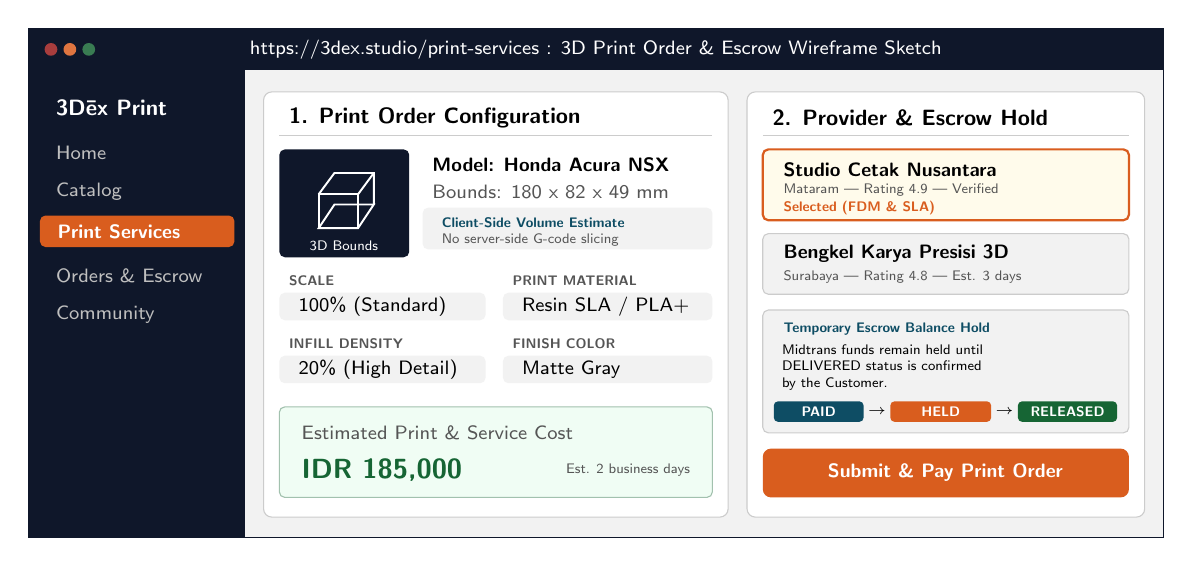
\begin{tikzpicture}[font=\sffamily]
    % Outer browser window frame (14.4cm width x 6.45cm height)
    \fill[white] (0,0) rectangle (14.4, 5.93);
    \fill[brandnavy] (0, 5.93) rectangle (14.4, 6.45);
    \fill[accentred!85!white] (0.28, 6.19) circle (2.3pt);
    \fill[accentorange!85!white] (0.52, 6.19) circle (2.3pt);
    \fill[accentgreen!85!white] (0.76, 6.19) circle (2.3pt);
    \node[anchor=center, font=\sffamily\scriptsize, text=white] at (7.2, 6.19) {https://3dex.studio/print-services : 3D Print Order \& Escrow Wireframe Sketch};
    \draw[brandnavy, line width=0.9pt] (0,0) rectangle (14.4, 6.45);

    % Left sidebar (2.75cm)
    \fill[brandnavy] (0,0) rectangle (2.75, 5.93);
    \node[anchor=west, font=\sffamily\footnotesize\bfseries, text=white] at (0.22, 5.45) {3D\={e}x Print};
    \node[anchor=west, font=\sffamily\scriptsize, text=gray!50] at (0.22, 4.88) {Home};
    \node[anchor=west, font=\sffamily\scriptsize, text=gray!50] at (0.22, 4.38) {Catalog};
    \fill[accentorange, rounded corners=2pt] (0.14, 3.68) rectangle (2.61, 4.08);
    \node[anchor=west, font=\sffamily\scriptsize\bfseries, text=white] at (0.24, 3.88) {Print Services};
    \node[anchor=west, font=\sffamily\scriptsize, text=gray!50] at (0.22, 3.32) {Orders \& Escrow};
    \node[anchor=west, font=\sffamily\scriptsize, text=gray!50] at (0.22, 2.82) {Community};

    % Main background area
    \fill[lightslate] (2.75, 0) rectangle (14.4, 5.93);

    % Left Content Card (width 5.90cm: x=2.98..8.88)
    \fill[white, rounded corners=3pt] (2.98, 0.25) rectangle (8.88, 5.65);
    \draw[bordergray, rounded corners=3pt] (2.98, 0.25) rectangle (8.88, 5.65);
    \node[anchor=west, font=\sffamily\footnotesize\bfseries, text=black] at (3.18, 5.32) {1. Print Order Configuration};
    \draw[bordergray] (3.18, 5.10) -- (8.68, 5.10);

    % Mini 3D Preview box (width 1.65cm: x=3.18..4.83)
    \fill[brandnavy, rounded corners=2pt] (3.18, 3.55) rectangle (4.83, 4.92);
    \draw[white!80, line width=0.7pt] (3.68, 3.92) -- (4.18, 3.92) -- (4.38, 4.22) -- (3.88, 4.22) -- cycle;
    \draw[white!80, line width=0.7pt] (3.68, 3.92) -- (3.68, 4.35) -- (4.18, 4.35) -- (4.18, 3.92);
    \draw[white!80, line width=0.7pt] (3.68, 4.35) -- (3.88, 4.62) -- (4.38, 4.62) -- (4.38, 4.22);
    \draw[white!80, line width=0.7pt] (4.18, 4.35) -- (4.38, 4.62);
    \node[anchor=center, font=\sffamily\tiny, text=white] at (4.00, 3.70) {3D Bounds};

    % Model summary next to box (width 3.68cm: x=5.00..8.68)
    \node[anchor=west, font=\sffamily\scriptsize\bfseries, text=black] at (5.00, 4.72) {Model: Honda Acura NSX};
    \node[anchor=west, font=\sffamily\scriptsize, text=mutedtext] at (5.00, 4.38) {Bounds: 180 x 82 x 49 mm};
    \fill[lightslate, rounded corners=2pt] (5.00, 3.65) rectangle (8.68, 4.18);
    \node[anchor=west, font=\sffamily\tiny\bfseries, text=accentteal] at (5.12, 3.99) {Client-Side Volume Estimate};
    \node[anchor=west, font=\sffamily\tiny, text=mutedtext] at (5.12, 3.77) {No server-side G-code slicing};

    % Parameters grid
    \node[anchor=west, font=\sffamily\tiny\bfseries, text=mutedtext] at (3.18, 3.25) {SCALE};
    \fill[lightslate, rounded corners=2pt] (3.18, 2.75) rectangle (5.80, 3.10);
    \node[anchor=west, font=\sffamily\scriptsize, text=black] at (3.30, 2.92) {100\% (Standard)};

    \node[anchor=west, font=\sffamily\tiny\bfseries, text=mutedtext] at (6.02, 3.25) {PRINT MATERIAL};
    \fill[lightslate, rounded corners=2pt] (6.02, 2.75) rectangle (8.68, 3.10);
    \node[anchor=west, font=\sffamily\scriptsize, text=black] at (6.14, 2.92) {Resin SLA / PLA+};

    \node[anchor=west, font=\sffamily\tiny\bfseries, text=mutedtext] at (3.18, 2.45) {INFILL DENSITY};
    \fill[lightslate, rounded corners=2pt] (3.18, 1.95) rectangle (5.80, 2.30);
    \node[anchor=west, font=\sffamily\scriptsize, text=black] at (3.30, 2.12) {20\% (High Detail)};

    \node[anchor=west, font=\sffamily\tiny\bfseries, text=mutedtext] at (6.02, 2.45) {FINISH COLOR};
    \fill[lightslate, rounded corners=2pt] (6.02, 1.95) rectangle (8.68, 2.30);
    \node[anchor=west, font=\sffamily\scriptsize, text=black] at (6.14, 2.12) {Matte Gray};

    % Estimated Total Footer
    \fill[softgreen, rounded corners=2pt] (3.18, 0.50) rectangle (8.68, 1.65);
    \draw[accentgreen!40, rounded corners=2pt] (3.18, 0.50) rectangle (8.68, 1.65);
    \node[anchor=west, font=\sffamily\scriptsize, text=mutedtext] at (3.34, 1.32) {Estimated Print \& Service Cost};
    \node[anchor=west, font=\sffamily\normalsize\bfseries, text=accentgreen] at (3.34, 0.85) {IDR 185,000};
    \node[anchor=east, font=\sffamily\tiny, text=mutedtext] at (8.52, 0.85) {Est. 2 business days};

    % Right Content Card (width 5.05cm: x=9.12..14.17)
    \fill[white, rounded corners=3pt] (9.12, 0.25) rectangle (14.17, 5.65);
    \draw[bordergray, rounded corners=3pt] (9.12, 0.25) rectangle (14.17, 5.65);
    \node[anchor=west, font=\sffamily\footnotesize\bfseries, text=black] at (9.32, 5.32) {2. Provider \& Escrow Hold};
    \draw[bordergray] (9.32, 5.10) -- (13.97, 5.10);

    % Selected Provider Card
    \fill[softamber, rounded corners=2pt] (9.32, 4.02) rectangle (13.97, 4.92);
    \draw[accentorange, line width=0.8pt, rounded corners=2pt] (9.32, 4.02) rectangle (13.97, 4.92);
    \node[anchor=west, font=\sffamily\scriptsize\bfseries, text=black] at (9.46, 4.66) {Studio Cetak Nusantara};
    \node[anchor=west, font=\sffamily\tiny, text=mutedtext] at (9.46, 4.40) {Mataram | Rating 4.9 | Verified};
    \node[anchor=west, font=\sffamily\tiny\bfseries, text=accentorange] at (9.46, 4.18) {Selected (FDM \& SLA)};

    % Alternate Provider Card
    \fill[lightslate, rounded corners=2pt] (9.32, 3.08) rectangle (13.97, 3.85);
    \draw[bordergray, rounded corners=2pt] (9.32, 3.08) rectangle (13.97, 3.85);
    \node[anchor=west, font=\sffamily\scriptsize\bfseries, text=black] at (9.46, 3.60) {Bengkel Karya Presisi 3D};
    \node[anchor=west, font=\sffamily\tiny, text=mutedtext] at (9.46, 3.30) {Surabaya | Rating 4.8 | Est. 3 days};

    % Escrow Flow Notice Box
    \fill[lightslate, rounded corners=2pt] (9.32, 1.32) rectangle (13.97, 2.88);
    \draw[bordergray, rounded corners=2pt] (9.32, 1.32) rectangle (13.97, 2.88);
    \node[anchor=west, font=\sffamily\tiny\bfseries, text=accentteal] at (9.46, 2.64) {Temporary Escrow Balance Hold};
    \node[anchor=west, align=left, font=\sffamily\tiny, text=black] at (9.44, 2.15) {Midtrans funds remain held until\\DELIVERED status is confirmed\\by the Customer.};
    \fill[accentteal, rounded corners=1.5pt] (9.46, 1.46) rectangle (10.60, 1.72);
    \node[font=\sffamily\tiny\bfseries, text=white] at (10.03, 1.59) {PAID};
    \node[font=\sffamily\tiny, text=black] at (10.77, 1.59) {$\rightarrow$};
    \fill[accentorange, rounded corners=1.5pt] (10.94, 1.46) rectangle (12.22, 1.72);
    \node[font=\sffamily\tiny\bfseries, text=white] at (11.58, 1.59) {HELD};
    \node[font=\sffamily\tiny, text=black] at (12.39, 1.59) {$\rightarrow$};
    \fill[accentgreen, rounded corners=1.5pt] (12.56, 1.46) rectangle (13.82, 1.72);
    \node[font=\sffamily\tiny\bfseries, text=white] at (13.19, 1.59) {RELEASED};

    % Primary Action Button
    \fill[accentorange, rounded corners=3pt] (9.32, 0.50) rectangle (13.97, 1.12);
    \node[anchor=center, font=\sffamily\scriptsize\bfseries, text=white] at (11.64, 0.81) {Submit \& Pay Print Order};
\end{tikzpicture}
\caption{Wireframe Sketch for Physical 3D Print Configuration, Volume Estimation, and Escrow Hold}
\end{figure}

\clearpage

% ==============================================================================
% APPENDIX B: STAKEHOLDER REGISTER & POWER/INTEREST GRID
% ==============================================================================
\section{Stakeholder Register (Process 13.1) and Power/Interest Grid}

\subsection{Stakeholder Register}
In alignment with PMBOK\textsuperscript{\textregistered} Guide 6th Edition Process 13.1 Identify Stakeholders, the table below maps project roles, interests, Power/Interest tiers, and engagement strategies:

\begin{table}[H]
\centering
\caption{3D\={e}x Project Stakeholder Register}
\footnotesize
\begin{tabularx}{\textwidth}{| L{2.7cm} | L{2.7cm} | L{3.6cm} | C{1.9cm} | Y |}
\hline
\rowcolor{tableheadergray} \thdr{Stakeholder} & \thdr{Project Role} & \thdr{Primary Interest} & \thdr{Power / Interest} & \thdr{Engagement Strategy} \\
\hline
Ir. Hendra Wijaya (Krea3D Corp) & Owner \& Executive Sponsor & Revenue growth, commercial ROI, schedule \& budget control & High / High & \textit{Manage Closely:} Engage on charter approval, scope changes, and final BAST. \\
\hline
Rina Kusumawardhani (Krea3D Corp) & On-Site Customer Representative & Smooth sales and printing workflows, operational ease & High / High & \textit{Manage Closely:} Attend every planning session, bi-weekly demo, and UAT sign-off. \\
\hline
3D\={e}x Engineering Team (PT SDN, 4 Staff) & Execution Team (PM, FE, BE, Integ., BA) & Clear requirements, structured modules, Day 106 delivery & Medium / High & \textit{Keep Informed / Core Sync:} Regular stand-ups, peer reviews, and integration checks. \\
\hline
Course Lecturer (Santi Ika Murpratiwi) & Academic Supervisor \& Evaluator & PMBOK 6 compliance, XP/PXP execution, charter quality & High / Medium & \textit{Keep Satisfied:} Deliver Charter drafts and milestone progress updates. \\
\hline
3D Digital Artists & Content Supply End Users & Fair monetization, license control, clear sales analytics & Low / High & \textit{Keep Informed:} Invite to UAT testing for model upload and creator dashboards. \\
\hline
3D Print Providers & Physical Production Partners & Accurate print sizing, organized job queues, escrow safety & Low / High & \textit{Keep Informed:} Involve in Provider Dashboard UAT and shipping entry tests. \\
\hline
End Customers & Asset Buyers \& Print Requesters & Smooth 3D previewing, escrow safety, accurate search results & Low / Medium & \textit{Monitor:} Collect beta UX feedback and monitor page response times. \\
\hline
Platform Administrators & Trust \& Safety Moderators & Proactive content screening and complete audit records & Medium / Medium & \textit{Keep Informed:} Provide moderation and dispute handling training before launch. \\
\hline
Third-Party Vendors (Midtrans, Google) & Payment, AI \& Cloud Providers & Service availability, transaction safety, quota stability & High / Low & \textit{Keep Satisfied / Monitor:} Track service status and adhere to vendor SLAs. \\
\hline
\end{tabularx}
\end{table}

\subsection{Power / Interest Grid and Communication Strategy}

\begin{figure}[H]
\centering
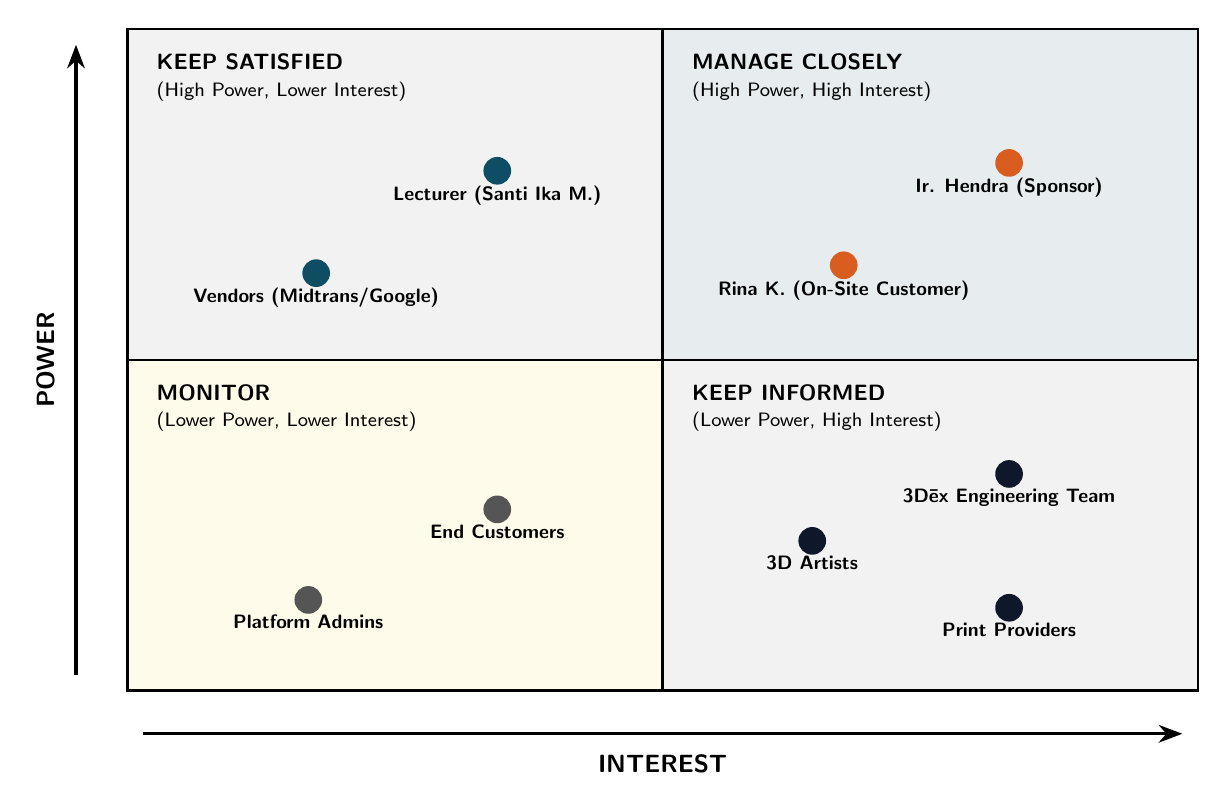
\begin{tikzpicture}[font=\sffamily\footnotesize]
    \fill[lightslate] (0,4.2) rectangle (6.8,8.4);
    \fill[accentteal!10] (6.8,4.2) rectangle (13.6,8.4);
    \fill[softamber] (0,0) rectangle (6.8,4.2);
    \fill[lightslate] (6.8,0) rectangle (13.6,4.2);

    \draw[black, line width=1pt] (0,0) rectangle (13.6,8.4);
    \draw[black, line width=0.9pt] (6.8,0) -- (6.8,8.4);
    \draw[black, line width=0.9pt] (0,4.2) -- (13.6,4.2);

    \node[anchor=north west, align=left, font=\sffamily\footnotesize, text=black] at (0.25, 8.2) {\textbf{KEEP SATISFIED}\\{\scriptsize (High Power, Lower Interest)}};
    \node[anchor=north west, align=left, font=\sffamily\footnotesize, text=black] at (7.05, 8.2) {\textbf{MANAGE CLOSELY}\\{\scriptsize (High Power, High Interest)}};
    \node[anchor=north west, align=left, font=\sffamily\footnotesize, text=black] at (0.25, 4.0) {\textbf{MONITOR}\\{\scriptsize (Lower Power, Lower Interest)}};
    \node[anchor=north west, align=left, font=\sffamily\footnotesize, text=black] at (7.05, 4.0) {\textbf{KEEP INFORMED}\\{\scriptsize (Lower Power, High Interest)}};

    \draw[-{Stealth[length=3mm]}, line width=1.1pt, black] (-0.65, 0.2) -- (-0.65, 8.2) node[midway, sloped, above=4pt, font=\sffamily\small\bfseries, text=black] {POWER};
    \draw[-{Stealth[length=3mm]}, line width=1.1pt, black] (0.2, -0.55) -- (13.4, -0.55) node[midway, below=4pt, font=\sffamily\small\bfseries, text=black] {INTEREST};

    \fill[accentorange] (11.2, 6.7) circle (5pt);
    \node[below=2pt, font=\sffamily\scriptsize\bfseries, text=black] at (11.2, 6.7) {Ir. Hendra (Sponsor)};

    \fill[accentorange] (9.1, 5.4) circle (5pt);
    \node[below=2pt, font=\sffamily\scriptsize\bfseries, text=black] at (9.1, 5.4) {Rina K. (On-Site Customer)};

    \fill[accentteal] (4.7, 6.6) circle (5pt);
    \node[below=2pt, font=\sffamily\scriptsize\bfseries, text=black] at (4.7, 6.6) {Lecturer (Santi Ika M.)};

    \fill[accentteal] (2.4, 5.3) circle (5pt);
    \node[below=2pt, font=\sffamily\scriptsize\bfseries, text=black] at (2.4, 5.3) {Vendors (Midtrans/Google)};

    \fill[brandnavy] (11.2, 2.75) circle (5pt);
    \node[below=2pt, font=\sffamily\scriptsize\bfseries, text=black] at (11.2, 2.75) {3D\={e}x Engineering Team};

    \fill[brandnavy] (8.7, 1.9) circle (5pt);
    \node[below=2pt, font=\sffamily\scriptsize\bfseries, text=black] at (8.7, 1.9) {3D Artists};

    \fill[brandnavy] (11.2, 1.05) circle (5pt);
    \node[below=2pt, font=\sffamily\scriptsize\bfseries, text=black] at (11.2, 1.05) {Print Providers};

    \fill[mutedtext] (4.7, 2.3) circle (5pt);
    \node[below=2pt, font=\sffamily\scriptsize\bfseries, text=black] at (4.7, 2.3) {End Customers};

    \fill[mutedtext] (2.3, 1.15) circle (5pt);
    \node[below=2pt, font=\sffamily\scriptsize\bfseries, text=black] at (2.3, 1.15) {Platform Admins};
\end{tikzpicture}
\caption{Stakeholder Power / Interest Grid Mapping}
\end{figure}

\begin{table}[H]
\centering
\caption{Stakeholder Communication Cadence and Channel Matrix}
\small
\begin{tabularx}{\textwidth}{| L{3.6cm} | L{3.0cm} | Y |}
\hline
\rowcolor{tableheadergray} \thdr{Strategic Quadrant} & \thdr{Cadence} & \thdr{Primary Channels \& Artifacts} \\
\hline
Manage Closely & Weekly / Per Phase & Planning sessions, bi-weekly sprint demos, formal change approvals, BAST. \\
\hline
Keep Satisfied & Per Milestone (M1 to M5) & Charter drafts, executive milestone reports, third-party service quota monitoring. \\
\hline
Keep Informed & Regular / Pre-Release & Daily team syncs, pre-release UAT testing workshops for Artists and Providers. \\
\hline
Monitor & Periodic / Post-Launch & Beta feedback surveys, content moderation queues, platform health logs. \\
\hline
\end{tabularx}
\end{table}

\clearpage

% ==============================================================================
% APPENDIX C: MILESTONE SCHEDULE, ITERATION PLAN & PERT BUDGET
% ==============================================================================
\section{Milestone Schedule, Iteration Plan, and PERT Budget Estimation}

\subsection{Hybrid Lifecycle (XP / PXP) and 15-Week Gantt Chart}
The 3D\={e}x project applies a Hybrid Lifecycle: scope, governance, and the fixed IDR 148,500,000 ceiling are baselined upfront, while software delivery proceeds through iterative Agile Extreme Programming (XP) and Personal Extreme Programming (PXP) cycles across five release phases over 106 calendar days.

\begin{figure}[H]
\centering
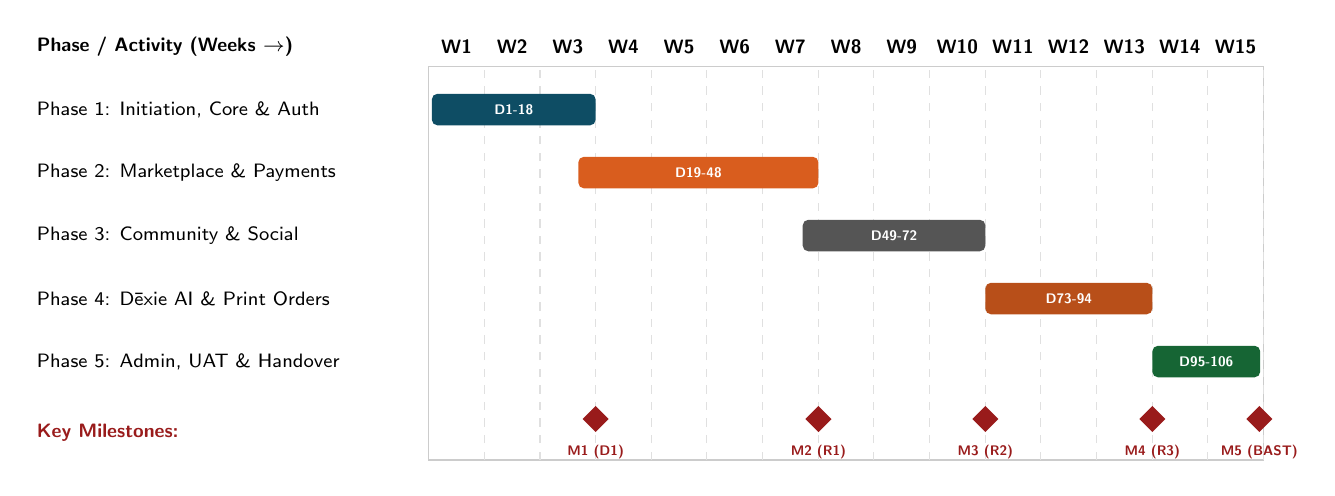
\begin{tikzpicture}[font=\sffamily\scriptsize]
    \draw[bordergray] (5.10, 0.2) rectangle (15.70, 5.2);
    \foreach \w in {1,...,15} {
        \pgfmathsetmacro{\xpos}{5.10 + (\w - 0.5) * (10.60 / 15)}
        \node[font=\sffamily\scriptsize\bfseries, text=black] at (\xpos, 5.45) {W\w};
        \draw[bordergray!60, dashed] ({5.10 + \w * (10.60/15)}, 0.2) -- ({5.10 + \w * (10.60/15)}, 5.2);
    }
    \node[anchor=west, font=\sffamily\scriptsize\bfseries, text=black] at (0, 5.45) {Phase / Activity (Weeks $\rightarrow$)};

    \node[anchor=west, text=black] at (0, 4.65) {Phase 1: Initiation, Core \& Auth};
    \fill[accentteal, rounded corners=2pt] (5.14, 4.45) rectangle (7.22, 4.85);
    \node[white, font=\sffamily\tiny\bfseries] at (6.18, 4.65) {D1-18};

    \node[anchor=west, text=black] at (0, 3.85) {Phase 2: Marketplace \& Payments};
    \fill[accentorange, rounded corners=2pt] (7.00, 3.65) rectangle (10.05, 4.05);
    \node[white, font=\sffamily\tiny\bfseries] at (8.525, 3.85) {D19-48};

    \node[anchor=west, text=black] at (0, 3.05) {Phase 3: Community \& Social};
    \fill[mutedtext, rounded corners=2pt] (9.85, 2.85) rectangle (12.17, 3.25);
    \node[white, font=\sffamily\tiny\bfseries] at (11.01, 3.05) {D49-72};

    \node[anchor=west, text=black] at (0, 2.25) {Phase 4: D\={e}xie AI \& Print Orders};
    \fill[accentorange!85!black, rounded corners=2pt] (12.17, 2.05) rectangle (14.29, 2.45);
    \node[white, font=\sffamily\tiny\bfseries] at (13.23, 2.25) {D73-94};

    \node[anchor=west, text=black] at (0, 1.45) {Phase 5: Admin, UAT \& Handover};
    \fill[accentgreen, rounded corners=2pt] (14.29, 1.25) rectangle (15.66, 1.65);
    \node[white, font=\sffamily\tiny\bfseries] at (14.975, 1.45) {D95-106};

    \node[anchor=west, font=\sffamily\scriptsize\bfseries, text=accentred] at (0, 0.55) {Key Milestones:};
    \foreach \x/\lbl in {7.22/M1 (D1), 10.05/M2 (R1), 12.17/M3 (R2), 14.29/M4 (R3), 15.65/M5 (BAST)} {
        \node[diamond, fill=accentred, inner sep=2.4pt] at (\x, 0.72) {};
        \node[below=1pt, font=\sffamily\tiny\bfseries, text=accentred] at (\x, 0.55) {\lbl};
    }
\end{tikzpicture}
\caption{15-Week (106-Day) Milestone Summary Schedule Aligned with XP Releases}
\end{figure}

\subsection{Iteration Plan and Core User Story Epics (Total: 106 Person-Days)}

\begin{table}[H]
\centering
\caption{Weekly Iteration Plan and User Story Allocation Across 5 Release Phases}
\small
\begin{tabularx}{\textwidth}{| C{1.6cm} | L{3.3cm} | Y | L{3.8cm} | C{1.3cm} |}
\hline
\rowcolor{tableheadergray} \thdr{Weeks} & \thdr{Phase / Iteration} & \thdr{Core Epics \& User Needs Addressed} & \thdr{Primary Actors} & \thdr{Est. (Pd)} \\
\hline
1 to 3 & Phase 1: Foundation & Charter sign-off, UI wireframes, registration, sign-in, and role access rules & All Actors & 11 \\
\hline
4 to 7 & Phase 2: Release 1 (Marketplace) & Public catalog, interactive 3D viewer, creator uploads, cart, Midtrans payment, secure downloads & Guest, Customer, Artist, Admin & 35 \\
\hline
8 to 10 & Phase 3: Release 2 (Community) & Creator portfolio feed, follow graph, verified buyer reviews, curated collections, notifications & Customer, Artist & 21 \\
\hline
11 to 13 & Phase 4: Release 3 (AI \& Print) & D\={e}xie smart discovery, physical print requests (\textit{bounding-box}), escrow hold, Provider Dashboard & Customer, Print Provider & 27 \\
\hline
14 to 15 & Phase 5: Final UAT \& Closure & Admin analytics, partner verification, audit logs, 100\% UAT, manuals, client training, handover & Admin, QA Team, Client & 12 \\
\hline
\rowcolor{lightslate} \multicolumn{4}{|r|}{\textbf{Total Estimated Effective Effort (5 Phases, Distributed Part-Time Team)}} & \textbf{106} \\
\hline
\end{tabularx}
\end{table}

\clearpage

\subsection{Three-Point (PERT), Parametric Calculations, and Cost Breakdown}
Engineering labor effort is calculated using PMBOK\textsuperscript{\textregistered} \textit{Three-Point Estimation (PERT)} ($E = \frac{O + 4M + P}{6}$ and $\sigma = \frac{P - O}{6}$), multiplied by PT Schryzon Digital Nusantara's commercial rate of IDR 1,000,000 per person-day.

\textit{Effort Capacity Note (106 Person-Days vs. 106 Calendar Days):}
The 106 person-days figure represents the cumulative effective engineering effort of the four-person student development team working on a distributed, part-time schedule (approximately 15 to 20 hours per week per person) across the 106-calendar-day (15-week) project timeline, rather than simultaneous full-time capacity.

\begin{table}[H]
\centering
\caption{PERT Effort and Parametric Engineering Cost Breakdown by Phase}
\small
\begin{tabularx}{\textwidth}{| Y | C{0.8cm} | C{0.8cm} | C{0.8cm} | C{1.6cm} | C{1.0cm} | R{3.1cm} |}
\hline
\rowcolor{tableheadergray} \thdr{Development Phase / Module} & \thdr{$O$} & \thdr{$M$} & \thdr{$P$} & \thdr{$E$ (Pd)} & \thdr{$\sigma$} & \thdr{Cost (Parametric)} \\
\hline
Phase 1: Foundation, Accounts \& Roles & 8 & 11 & 14 & 11.0 & 1.00 & IDR 11,000,000 \\
\hline
Phase 2: Marketplace \& Midtrans Checkout & 28 & 35 & 42 & 35.0 & 2.33 & IDR 35,000,000 \\
\hline
Phase 3: Community \& Social Features & 16 & 21 & 26 & 21.0 & 1.67 & IDR 21,000,000 \\
\hline
Phase 4: D\={e}xie AI \& Print Ecosystem & 20 & 27 & 34 & 27.0 & 2.33 & IDR 27,000,000 \\
\hline
Phase 5: Admin, UAT \& Handover & 9 & 12 & 15 & 12.0 & 1.00 & IDR 12,000,000 \\
\hline
\rowcolor{lightslate} \textbf{Total Engineering Effort (PERT)} & \textbf{81} & \textbf{106} & \textbf{131} & \textbf{106.0} & \textbf{8.33} & \textbf{IDR 106,000,000} \\
\hline
\end{tabularx}
\end{table}

\begin{table}[H]
\centering
\caption{Detailed Approved Budget Schedule (Sponsor Approved)}
\small
\begin{tabularx}{\textwidth}{| L{5.1cm} | Y | R{3.1cm} | C{1.4cm} |}
\hline
\rowcolor{tableheadergray} \thdr{Cost Component} & \thdr{Line-Item Details} & \thdr{Amount (IDR)} & \thdr{Share} \\
\hline
1. Software Engineering Labor & 106 person-days $\times$ IDR 1,000,000 (4 Part-Time Engineers) & IDR 106,000,000 & 71.38\% \\
\hline
2. Cloud Infrastructure \& APIs (12 Mo) & Production Hosting, File Storage, SSL, Gemini \& Midtrans APIs & IDR 16,500,000 & 11.11\% \\
\hline
3. UI/UX Design, 3D Tuning \& QA & Dark-Theme Assets, Viewer Performance \& Regression QA & IDR 7,500,000 & 5.05\% \\
\hline
4. Documentation, Training \& UAT & Handover Manuals, BAST \& Client Staff Training Workshop & IDR 5,000,000 & 3.37\% \\
\hline
\rowcolor{lightslate} \textbf{Baseline Cost Subtotal} & \textbf{Total Planned Direct Costs} & \textbf{IDR 135,000,000} & \textbf{90.91\%} \\
\hline
5. Risk Contingency Reserve & 10\% of Subtotal for Risks R-01 through R-07 & IDR 13,500,000 & 9.09\% \\
\hline
\rowcolor{lightslate} \textbf{TOTAL APPROVED BUDGET} & \textbf{Fixed Ceiling, PT Kreasi Tiga Dimensi Indonesia} & \textbf{IDR 148,500,000} & \textbf{100.00\%} \\
\hline
\end{tabularx}
\end{table}

\begin{figure}[H]
\centering
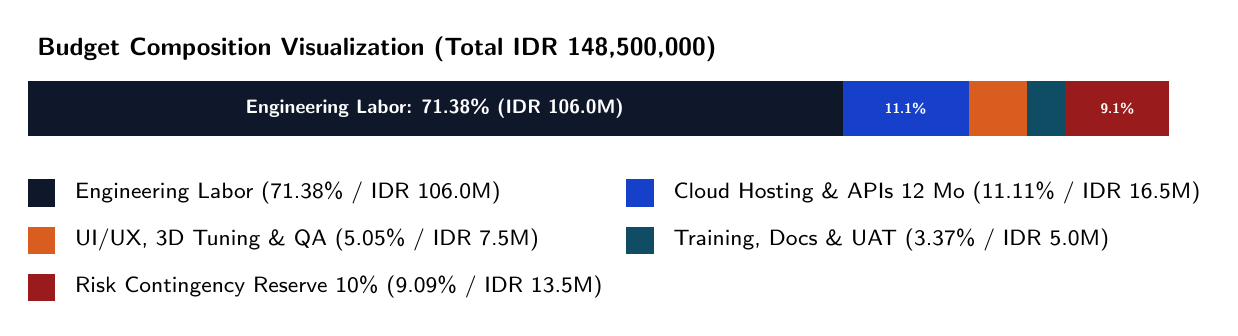
\begin{tikzpicture}[font=\sffamily\footnotesize]
    \node[anchor=west, font=\sffamily\small\bfseries, text=black] at (0, 3.3) {Budget Composition Visualization (Total IDR 148,500,000)};

    \fill[brandnavy] (0, 2.2) rectangle (10.35, 2.9);
    \fill[brandblue] (10.35, 2.2) rectangle (11.96, 2.9);
    \fill[accentorange] (11.96, 2.2) rectangle (12.69, 2.9);
    \fill[accentteal] (12.69, 2.2) rectangle (13.18, 2.9);
    \fill[accentred] (13.18, 2.2) rectangle (14.50, 2.9);

    \node[white, font=\sffamily\scriptsize\bfseries] at (5.17, 2.55) {Engineering Labor: 71.38\% (IDR 106.0M)};
    \node[white, font=\sffamily\tiny\bfseries] at (11.15, 2.55) {11.1\%};
    \node[white, font=\sffamily\tiny\bfseries] at (13.84, 2.55) {9.1\%};

    \fill[brandnavy] (0, 1.3) rectangle (0.35, 1.65);
    \node[anchor=west, text=black] at (0.48, 1.48) {Engineering Labor (71.38\% / IDR 106.0M)};

    \fill[brandblue] (7.6, 1.3) rectangle (7.95, 1.65);
    \node[anchor=west, text=black] at (8.08, 1.48) {Cloud Hosting \& APIs 12 Mo (11.11\% / IDR 16.5M)};

    \fill[accentorange] (0, 0.7) rectangle (0.35, 1.05);
    \node[anchor=west, text=black] at (0.48, 0.88) {UI/UX, 3D Tuning \& QA (5.05\% / IDR 7.5M)};

    \fill[accentteal] (7.6, 0.7) rectangle (7.95, 1.05);
    \node[anchor=west, text=black] at (8.08, 0.88) {Training, Docs \& UAT (3.37\% / IDR 5.0M)};

    \fill[accentred] (0, 0.1) rectangle (0.35, 0.45);
    \node[anchor=west, text=black] at (0.48, 0.28) {Risk Contingency Reserve 10\% (9.09\% / IDR 13.5M)};
\end{tikzpicture}
\caption{3D\={e}x Commercial Project Budget Allocation}
\end{figure}

\clearpage

% ==============================================================================
% APPENDIX D: RESOURCE INVENTORY & RACI MATRIX
% ==============================================================================
\section{Resource Inventory (Team, XP Roles \& Equipment) and RACI Matrix}

\subsection{Project Team and Extreme Programming (XP) Roles}

\begin{table}[H]
\centering
\caption{Core Team Roster, XP Roles, and Ownership Domains}
\begin{tabularx}{\textwidth}{| L{4.3cm} | C{2.3cm} | L{3.2cm} | Y |}
\hline
\rowcolor{tableheadergray} \thdr{Team Member} & \thdr{ID / NIM} & \thdr{XP Role} & \thdr{Primary Ownership Domain} \\
\hline
I Nyoman Widiyasa Jayananda & F1D02410053 & PM / Tracker \& Programmer & Iteration leadership, core backend services, central database, 3D storage pipeline, D\={e}xie AI discovery, and release governance. \\
\hline
I Kadek Mahesa Permana Putra & F1D02410052 & Programmer \& Tester (QA Lead) & Web interface pages, dark-theme UI system, interactive browser 3D viewer, and regression / UAT quality testing. \\
\hline
Abdurrahman Karim & F1D02410031 & Programmer & UI-to-backend integration, Google sign-in flow, Midtrans checkout integration, physical 3D print workflow (\textit{escrow}), and alerts. \\
\hline
Fido Priasa Setyono Putra & F1D02410048 & Customer Liaison / Analyst & Business analysis, Project Charter and UML documentation, UAT coordination, and client staff training delivery. \\
\hline
Rina Kusumawardhani (Krea3D Corp) & KREA3D-PO & On-Site Customer & Feature prioritization across planning cycles, sprint demo validation, and final UAT acceptance. \\
\hline
\end{tabularx}
\end{table}

\subsection{Hardware, Software, and Infrastructure Inventory}
\begin{itemize}[leftmargin=1.5em, itemsep=2pt]
    \item \textit{Engineering Hardware:} 4 Development Workstations with multi-core CPUs, 16 to 32 GB RAM, and WebGL-capable GPUs for local development and 3D verification.
    \item \textit{Software \& Collaboration Tools:} Integrated code editors, private version-controlled repositories, local web/database environments, and structured document preparation tools.
    \item \textit{Testing \& Production Hosting:} Cloud hosting for the web application and 3D storage, paired with sandbox/production accounts for Midtrans payments and Google AI services.
\end{itemize}

\subsection{Responsibility Assignment Matrix (RACI Matrix)}
Legend: \textbf{R} = \textit{Responsible}, \textbf{A} = \textit{Accountable} (strictly one single Accountable per row), \textbf{C} = \textit{Consulted}, \textbf{I} = \textit{Informed}. Under strict RACI governance, every activity assigns a pure \textbf{A} separate from \textbf{R} executors without mixing \textit{A/R} in the same cell.

\begin{table}[H]
\centering
\caption{RACI Matrix Across Core Project Domains}
\footnotesize
\begin{tabularx}{\textwidth}{| Y | C{1.55cm} | C{1.55cm} | C{1.55cm} | C{1.55cm} | C{1.85cm} |}
\hline
\rowcolor{tableheadergray} \thdr{Project Activity / Domain} & \thdr{Jay (PM/BE)} & \thdr{Mahesa (FE/QA)} & \thdr{Karim (Integ.)} & \thdr{Fido (BA/Doc)} & \thdr{Rina (Cust.)} \\
\hline
1. Project Charter v1.0 Authoring & \textbf{A} & C & C & R & C \\
\hline
2. User Story Writing \& Prioritization & R & C & C & R & \textbf{A} \\
\hline
3. Database Design \& System Structure & \textbf{A} & I & R & C & I \\
\hline
4. Core Backend Service Development & \textbf{A} & C & R & I & I \\
\hline
5. Web Interface \& Interactive 3D Viewer & C & \textbf{A} & R & I & C \\
\hline
6. Account Security, Google Login \& Roles & \textbf{A} & I & R & I & I \\
\hline
7. Midtrans Payment Integration & \textbf{A} & I & R & I & C \\
\hline
8. 3D Asset Storage \& Timed Downloads & \textbf{A} & I & R & I & I \\
\hline
9. D\={e}xie AI Smart Search \& Picks & \textbf{A} & R & I & I & C \\
\hline
10. Print Order (\textit{Escrow}) \& Provider Dashboard & \textbf{A} & C & R & C & C \\
\hline
11. Community Feed, Reviews \& Notifications & \textbf{A} & C & R & I & I \\
\hline
12. Admin Moderation \& Audit Logging & \textbf{A} & C & R & C & I \\
\hline
13. Regression, Performance \& UAT Testing & C & \textbf{A} & R & R & C \\
\hline
14. Release Demo, Training \& Final Handover & \textbf{A} & R & R & R & C / Approver \\
\hline
\end{tabularx}
\end{table}

\end{document}
